\documentclass[10pt, a4j, dvipdfmx]{jarticle}
\usepackage{titlesec}
\usepackage[dvipdfmx]{graphicx}
\usepackage[dvipdfmx]{color}
\usepackage{float}
\usepackage{wrapfig}
\usepackage{subfigure}
\usepackage{caption}
\usepackage{multirow}

\graphicspath{{../images/}}

\makeatletter
\newcommand{\figcaption}[1]{\def\@captype{figure}\caption{#1}}
\newcommand{\tblcaption}[1]{\def\@captype{table}\caption{#1}}
\makeatother

\title{トランジスタ増幅}
\author{4年 電子システム工学科 40番  山地 駿徹}


\begin{document}
    \section{実験方法}
    \subsection{トランジスタの静特性}

    \subsubsection{入力特性の測定方法}
    エミッタ接地回路で,$V_{CE}$を一定に保ち,$V_{BE}$を変化させたときの$I_B$の変化を測定する.
    \begin{figure}[H]
        \begin{minipage}{0.5\hsize}
            \centering
            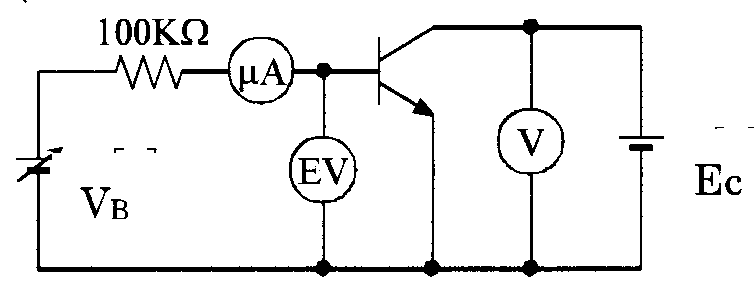
\includegraphics[width=50mm]{fig-1.png}
            \caption{入力特性測定回路}
            \label{fig:1}
        \end{minipage}
        \begin{minipage}{0.5\hsize}
            \centering
            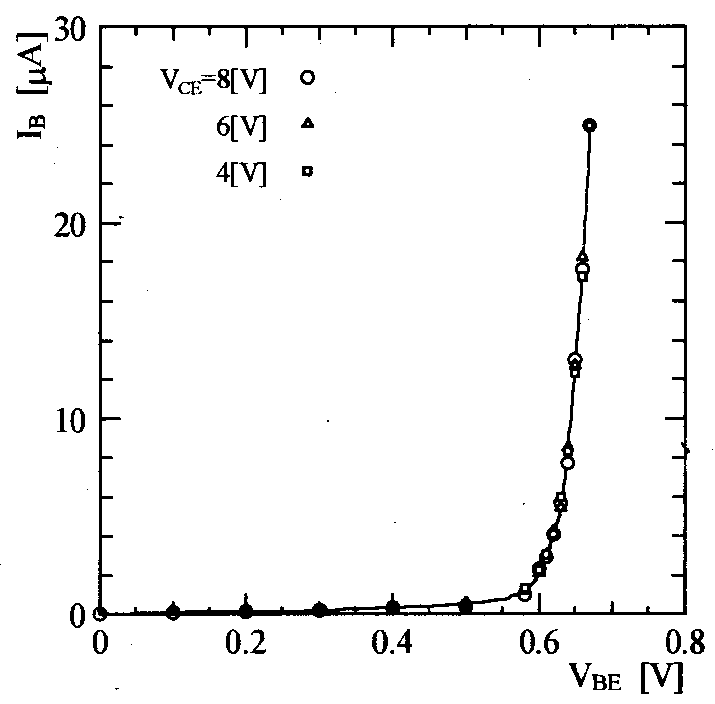
\includegraphics[height=45mm]{fig-2.png}
            \caption{入力特性}
            \label{fig:2}
        \end{minipage}
    \end{figure}

    \subsubsection{出力特性の測定方法}
    エミッタ接地回路で,$I_B$を一定に保ち,$V_{CE}$を変化させたときの$I_C$の変化を測定する.
    \begin{figure}[H]
        \begin{minipage}{0.5\hsize}
            \centering
            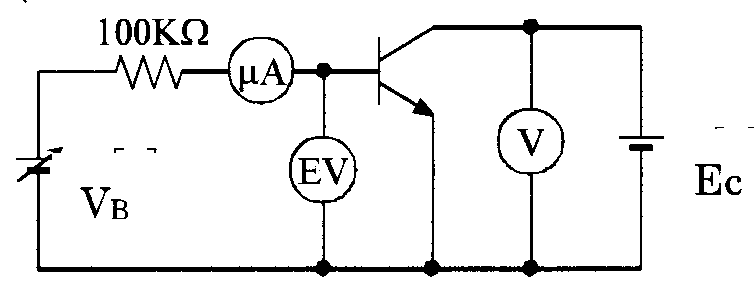
\includegraphics[width=50mm]{fig-1.png}
            \caption{出力特性測定回路}
            \label{fig:3}
        \end{minipage}
        \begin{minipage}{0.5\hsize}
            \centering
            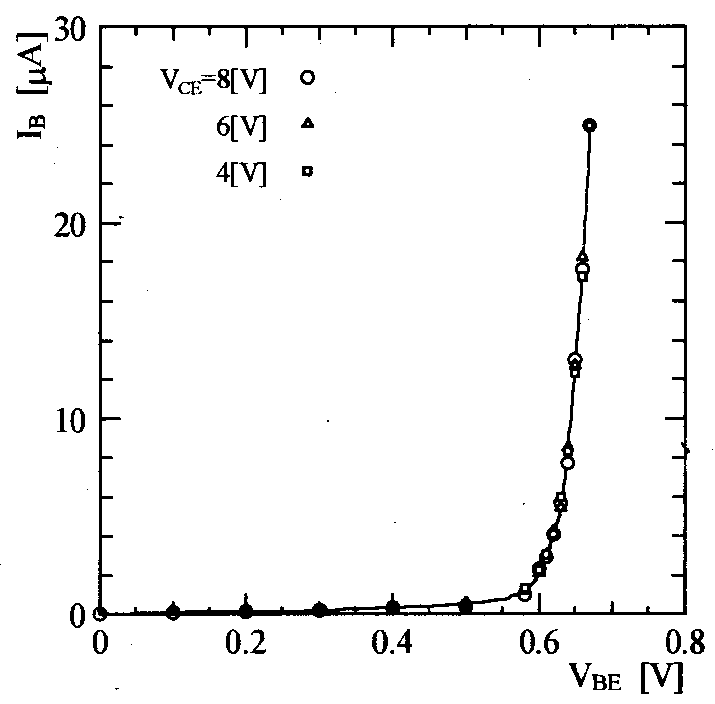
\includegraphics[height=45mm]{fig-2.png}
            \caption{出力特性}
            \label{fig:4}
        \end{minipage}
    \end{figure}
    \subsubsection{吟味事項}
    \begin{enumerate}
        \item 電圧計,電流計の等級と内部抵抗を調べる.\\電圧計,電流計の接続方法により,計器の内部抵抗による測定誤差について考察する.\\その時の補正方法を考察する.
        \item $V_{CE} = 4[V]$,$I_B = 20[\mu A]$のときの$h$定数を,測定した特性図より求める.
    \end{enumerate}

    \newpage
    \subsection{トランジスタ増幅}

    \subsubsection{電流増幅特性の測定方法}
    エミッタ接地回路で$R_C = 1[k\Omega]$を接続し$E_C = 8[V]$一定として,$I_B$を変化させたときの$I_C$の変化を測定する.
    \small (注. 電流計の内部抵抗が負荷抵抗に加算されないように$E_C$を調整する)
    \normalsize
    \begin{figure}[H]
        \begin{minipage}{0.5\hsize}
            \centering
            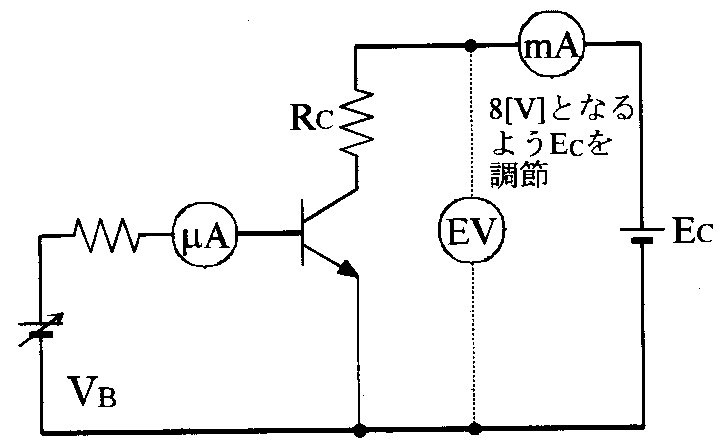
\includegraphics[width=50mm]{fig-5.png}
            \caption{電流増幅特性測定回路}
            \label{fig:5}
        \end{minipage}
        \begin{minipage}{0.5\hsize}
            \centering
            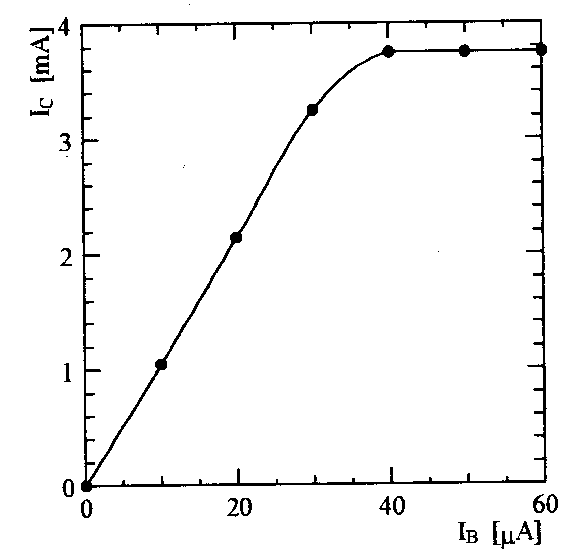
\includegraphics[height=45mm]{fig-6.png}
            \caption{電流増幅特性}
            \label{fig:6}
        \end{minipage}
    \end{figure}

    \subsubsection{電圧増幅特性の測定方法}
    エミッタ接地回路で$R_C = 1[k\Omega]$を接続し$E_C = 8[V]$一定として,$V_{BE}$を変化させたときの$V_{CE}$の変化を測定する.
    \begin{figure}[H]
        \begin{minipage}{0.5\hsize}
            \centering
            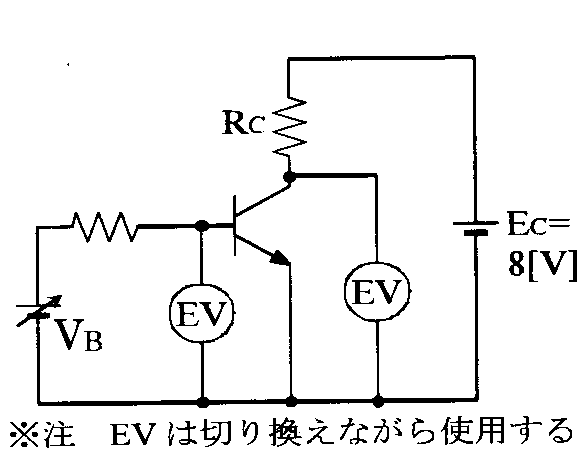
\includegraphics[width=50mm]{fig-7.png}
            \caption{電圧増幅特性測定回路}
            \label{fig:7}
        \end{minipage}
        \begin{minipage}{0.5\hsize}
            \centering
            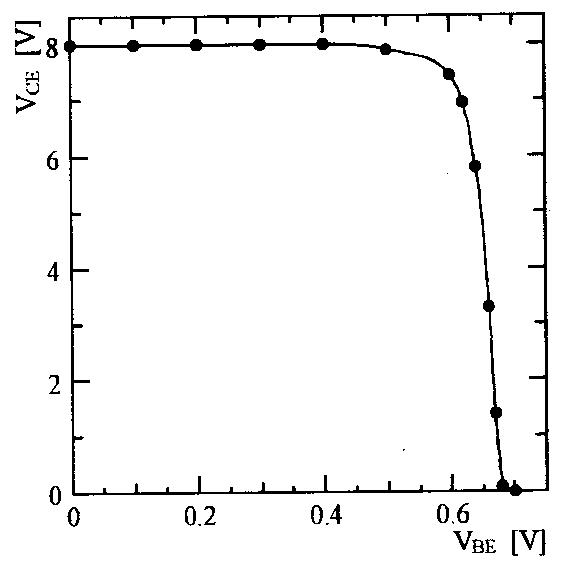
\includegraphics[height=45mm]{fig-8.png}
            \caption{電圧増幅特性}
            \label{fig:8}
        \end{minipage}
    \end{figure}

    以上の測定はトランジスタ増幅回路の交流不可線上の特性を測定することと等価である.\\
    まず,動作点$Q$を電流増幅特性の直線部分より決定する.次に,この動作点に対応する電圧増幅特性での動作点を記入する.

    \subsubsection{吟味事項}
    \begin{enumerate}
        \item 電流増幅特性より,$h_{FE}$を求める.
        \item 電圧増幅特性より電圧増幅度を求める.
    \end{enumerate}

    \newpage
    \subsubsection{直流バイアス回路定数の選定及びバイアス電圧測定}
    \begin{wrapfigure}{r}{70mm}
        \vspace*{-\intextsep}
        \begin{center}
            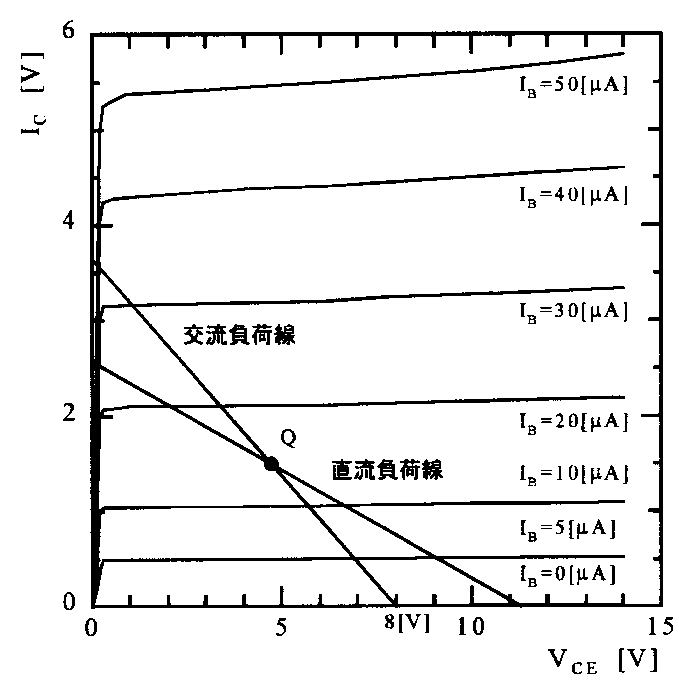
\includegraphics[height=50mm]{fig-9.png}
            \label{fig:9}
            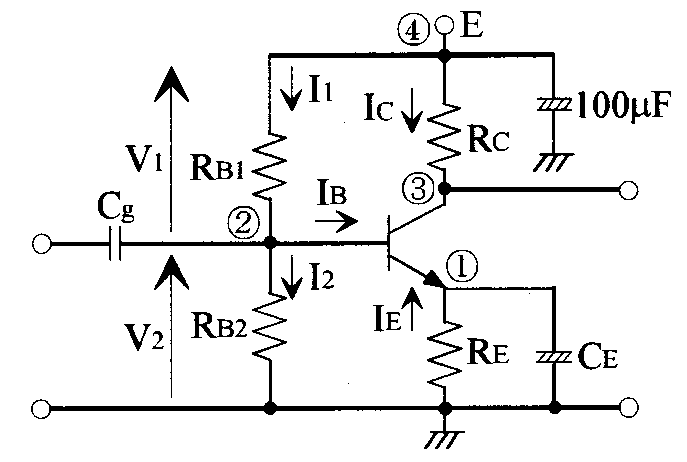
\includegraphics[height=40mm]{fig-10.png}
            \caption{出力特性測定回路}
            \label{fig:10}
        \end{center}
    \end{wrapfigure}
    先の実験で測定した出力特性に$8[V]$,$R_C$の交流負荷線を引き,動作点を記入する.\\ 
    \begin{equation}
        E_C = R_C I_C + V_{CE}
    \end{equation}
    また,動作点を通る傾き$1/(R_C + R_E)$の直流負荷線を引き,電源電圧を決定する.\\
    ここでは$R_C = R_E = 1k\Omega$とする.

    以下の下線部を埋めて実験を行う.\\
    Trの名称\hspace{25mm}\underline{\hspace{30mm}}\\
    交流負荷線 $R_C = $    \underline{\hspace{20mm}}$\Omega$\\
    直流負荷線 $R_C + R_E = $  \underline{\hspace{20mm}}$\Omega$\\
               $R_E = $     \underline{\hspace{20mm}}$\Omega$\\
    \\
    電源電圧 $E = $ \underline{\hspace{20mm}}$V$\\
    設定した動作点Qにおける\\
    ベース電流 $I_{BQ} = $ \underline{\hspace{20mm}}$\mu A$\\
    コレクタ電流 $I_{CQ} = $ \underline{\hspace{20mm}}$mA$\\
    電流増幅率 \underline{\hspace{20mm}}\\
    ベース-エミッタ間電圧 $V_{BEQ} = $ \underline{\hspace{20mm}}$V$\\
    コレクタ-エミッタ間電圧 $V_{CEQ} = $ \underline{\hspace{20mm}}$V$\\
    \\
    静特性から,図\ref{fig:10}における各点の電位は,\\
    \hspace{7mm}\textcircled{\scriptsize 1} \underline{\hspace{20mm}}$V$\hspace{7mm}\textcircled{\scriptsize 2} \underline{\hspace{20mm}}$V$\hspace{7mm}\textcircled{\scriptsize 3} \underline{\hspace{20mm}}$V$\\
    また,$I_2 = V_2 / R_{B2}$,$I_1 = (E - V_2)$,$I_1 = I_2 + I_{BQ}$の関係が成り立つ.\\
    $I_{BQ}$,$V_1$,$V_2$,$E$は既知である.また,係数$k$を導入し,$I_2 = k I_{BQ}$と表す.これらを用いて$I_1$,$I_2$,$R_{B1}$,$R_{B2}$を式で表すと\\
    \hspace{7mm}$I_1 = $ \underline{\hspace{20mm}}\hspace{7mm}$I_2 = $ \underline{\hspace{20mm}}\hspace{7mm}$R_{B1} = $ \underline{\hspace{20mm}}$R_{B2} = $ \underline{\hspace{20mm}}\\
    となる.$k$の値を変えていくつかの場合について$R_{B1}$,$R_{B2}$の値を求めよ.一番右端の欄には,実験回路に選んだ値を記せ.
    \begin{table}[H]
        \begin{tabular}{||c||c|c|c|c|c|c||c||}
        \hline\hline
        $k$      & $1$           & $5$           & $10$          &               &               &               &               \\ \hline\hline
        $R_{B1}$ & \hspace{15mm} & \hspace{15mm} & \hspace{15mm} & \hspace{15mm} & \hspace{15mm} & \hspace{15mm} & \hspace{15mm} \\ \hline
        $R_{B2}$ &               &               &               &               &               &               &               \\ \hline\hline
        \end{tabular}
    \end{table}
    \newpage
    増幅しようとする周波数範囲は,\hspace{7mm}\underline{\hspace{20mm}}$Hz$〜\hspace{7mm}\underline{\hspace{20mm}}$Hz$\\
    この下限周波数より,$C_g$,$C_E$を決定すると,$C_g = $\underline{\hspace{20mm}}$\mu A$\hspace{7mm} \underline{\hspace{20mm}}$\mu A$\\
    各点の電位及び電圧
    \begin{table}[H]
        \begin{tabular}{||c||c|c|c||c||c|c|c||}
        \hline\hline
        点                           & 設計値           & 実測値           & 誤差            & 点                                                           & 設計値           & 実測値           & 誤差            \\ \hline\hline
        \textcircled{\scriptsize 1} & \hspace{15mm} & \hspace{15mm} & \hspace{15mm} & $\textcircled{\scriptsize 3} - \textcircled{\scriptsize 1}$ & \hspace{15mm} & \hspace{15mm} & \hspace{15mm} \\ \hline
        \textcircled{\scriptsize 2} &               &               &               & $\textcircled{\scriptsize 2} - \textcircled{\scriptsize 1}$ &               &               &               \\ \hline
        \textcircled{\scriptsize 3} &               &               &               & $\textcircled{\scriptsize 4} - \textcircled{\scriptsize 2}$ &               &               &               \\ \hline
        \textcircled{\scriptsize 4} &               &               &               & $\textcircled{\scriptsize 4} - \textcircled{\scriptsize 3}$ &               &               &               \\ \hline\hline
        \end{tabular}
    \end{table}

    \subsubsection*{補足:直流バイアス回路の設計}
    \begin{wrapfigure}{r}{30mm}
        \vspace*{-\intextsep}
        \begin{center}
            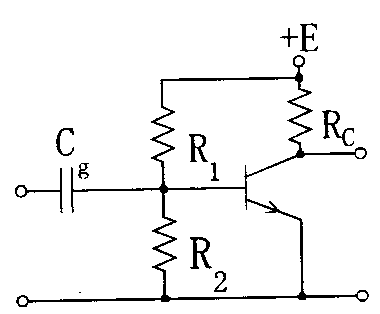
\includegraphics[width=30mm]{fig-11.png}
            \caption{}
            \label{fig:10}
        \end{center}
    \end{wrapfigure}
    トランジスタの静特性(出力特性)に交流負荷線$R_C$を引き,動作点$Q$を設定する.
    
    このとき,トランジスタに流れるベース電流$I_{BQ}$,コレクタ電流$I_{CQ}$,ベース-エミッタ間電圧$V_{BEQ}$,コレクタ-エミッタ間電圧$V_{CEQ}$をトランジスタの静特性より求める.

    求めた$I_{BEQ}$,$I_{CEQ}$が流れるように
    \begin{equation}
        V_2 = \{R_2 / (R_1 + R_2)\} E = V_{BEQ}
    \end{equation}
    から$R_1$,$R_2$の値を設定する.

    これで良いのであるが,トランジスタは温度によって特性が変化する.特性が変化すると設定した動作点qがずれてしまい増幅器の特性も安定しなくなる.\\
    \begin{wrapfigure}{r}{30mm}
        \vspace*{-\intextsep}
        \begin{center}
            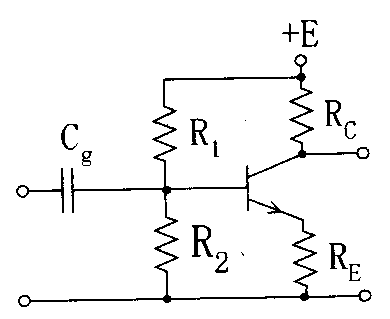
\includegraphics[width=30mm]{fig-12.png}
            \caption{}
            \label{fig:11}
        \end{center}.・
    \end{wrapfigure}.・
    そこで負帰還をかけて特性の変化による動作店の変動を.・抑制するため図\ref{fig:11}のように$R_E$を接続する.

    このとき,$R_C + R_E$は直流負荷線として図\ref{fig:9}のように静特性上に交流負荷線の動作点$Q$で交わる直線として引く.
    電源電圧$E$は$8V$から$R_E$による電圧降下分を加えた12Vに変わる.\\
    温度が交渉してベース電流が$I_{BQ}$よりも増加したとすると$R_E$による電圧降下は,
    \begin{equation}
        R_E(I_B + I_C) = R_E(I_{BQ} + I_{CQ} + \Delta I_B + \Delta I_C)
    \end{equation}\\
    となり,$R_E(\Delta I_B + \Delta I_C)$だけ$R_E$による電圧降下は大きくなる.\\
    $V_2$が一定であると仮定すると,
    \begin{equation}
        V_{BE} = V_2 - R_E(I_B + I_C) = V_2 - R_E(I_{BQ} + I_{CQ} + \Delta I_B + \Delta I_C)
    \end{equation}\\
    なので$I_B$が増加すると$V_{BE}$は小さくなる.$V_{BE}$が小さくなると$I_B$は減少する.
    このように$R_E$を接続することにより,ベース電流が増加(減少)しようとすると負帰還が働きベース電流の増加(減少)を押さえ,ベース電流を一定に保つ.

    次に,前述の解析では,$V_2$が一定であると仮定したわけであるが,$V_2$を一定にするためには,$R_2$にながれる電流$I_2$と$I_{BQ}$の比を大きくするとよい.
    $I_B$が増加するとその文だけ$I_2$は減少するが,比が大きいと$I_2$にとってその変化分はわずかな変化でしかなく,
    \begin{equation}
        V_2 = R_2 \cdot I_2 \approx 一定
    \end{equation}\\
    となる.

    今回の設計では,$I_ = k I_{BQ}$という定数$k$を導入する.
    $k$の値を大きくするほうが安定度は良いのであるだ,kを大きくしすぎると$R_1$と$R_2$の値が小さくなりすぎる.
    市販品の少抵抗は少なく,誤差も大きい.
    また,消費電力$R_2 \cdot I_2^2$が大きくなってよくない.
    消費電力が大きくなると発熱し,トランジスタの周囲温度を上げ,特性の変化をもたらす.\\
    \emph{ここでは,$R_1$と$R_2$の値は数$k\Omega$〜数$10k\Omega$程度になるように$k$を選ぶとよい.}

    \newpage
    \subsubsection{入出力特性の測定方法}
    設計製作した増幅回路に,低周波発振器より$f = 1kHz$の正弦波信号を入力する.
    この入力信号の入力電圧に対する出力電圧の変化を測定する.
    オシロスコープで入力波形と出力波形の変化も観測する.
    \begin{figure}[H]
        \begin{minipage}{0.5\hsize}
            \centering
            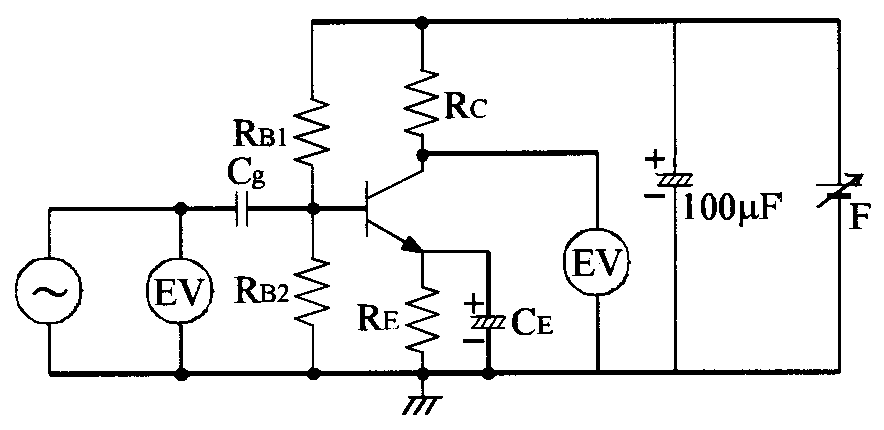
\includegraphics[width=50mm]{fig-13.png}
            \caption{入出力特性測定回路}
            \label{fig:12}
        \end{minipage}
        \begin{minipage}{0.5\hsize}
            \centering
            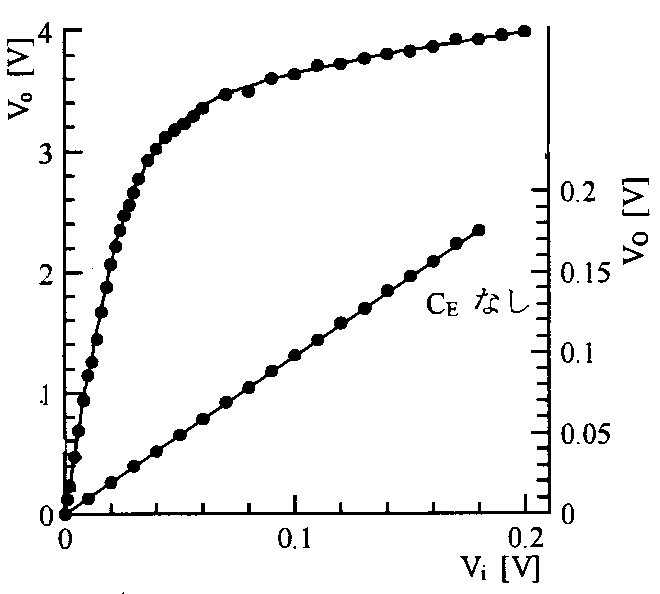
\includegraphics[height=45mm]{fig-14.png}
            \caption{入出力特性}
            \label{fig:13}
        \end{minipage}
    \end{figure}

    \subsubsection{周波数特性の測定}
    設計製作した増幅回路に,低周波発振器より正弦波信号を入力する.
    この入力信号の入力電圧を例えば$e_i = 10[mV]$一定にして,入力信号の周波数を変化させたときの出力電圧の変化を測定する.
    $C_E$の値を変えて同じ測定を行う.
    \begin{figure}[H]
        \begin{minipage}{0.5\hsize}
            \centering
            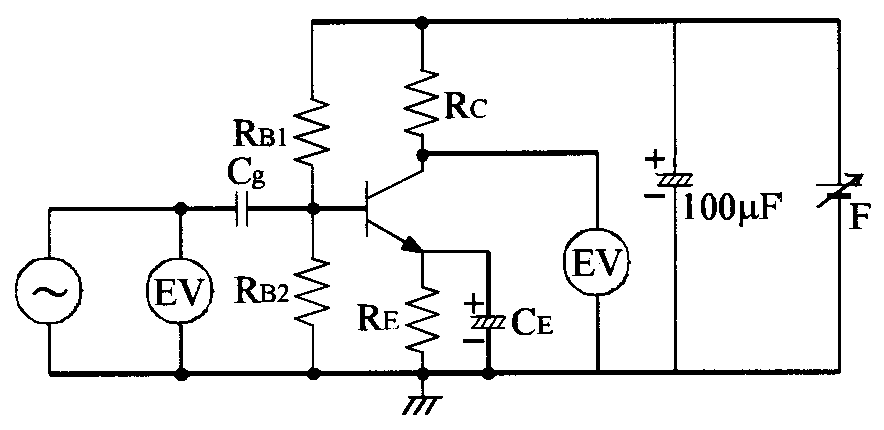
\includegraphics[width=50mm]{fig-15.png}
            \caption{周波数特性測定回路}
            \label{fig:14}
        \end{minipage}
        \begin{minipage}{0.5\hsize}
            \centering
            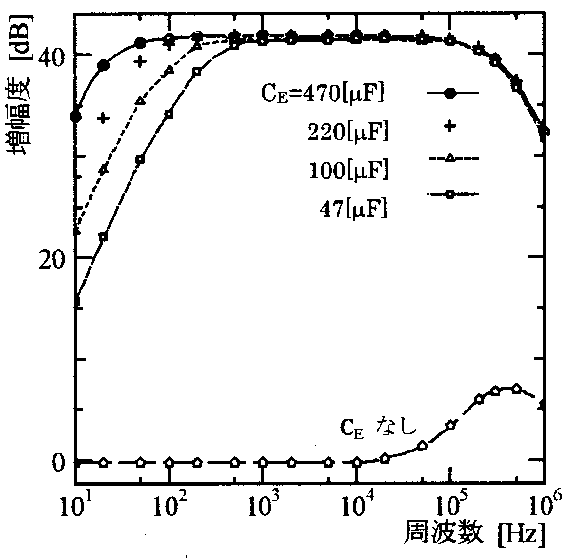
\includegraphics[height=45mm]{fig-16.png}
            \caption{周波数特性}
            \label{fig:15}
        \end{minipage}
    \end{figure}

    \subsubsection{吟味事項}
    \begin{enumerate}
        \item 入出力特性より,制作した増幅回路の増幅度を求める.
        \item バイパスコンデンサ$C_E$のない回路について解析する.測定はしなくていい.
        \item 観測した入力波形および出力波形について,入力特性や増幅特性をもとに考察する.
    \end{enumerate}

    \newpage
    \section{実験結果の処理}
    \subsection{トランジスタの静特性}

    \subsubsection{入力特性の測定結果}
    1.1.1に示した測定を,同一種のトランジスタ3個について,それぞれ行った.
    それぞれを$Tr_1$,$Tr_2$,$Tr_3$と区別することとする.

    以下表\ref{tbl:1}に$Tr_1$の測定結果の表を,図\ref{ex:1}に$Tr_1$の測定結果のグラフを示す.
    \begin{table}[H]
        \centering
        \caption{$Tr_1$の入力特性の測定値}
        \label{tbl:1}
        \small
        \begin{tabular}{|l|l|l|l|l|l|}
        \hline
        \multirow{2}{*}{$V_{BE}[V]$} & $V_{CE}=4[V]$ & \multirow{2}{*}{$V_{BE}[V]$} & $V_{CE}=6[V]$ & \multirow{2}{*}{$V_{BE}[V]$} & $V_{CE}=8[V]$ \\ \cline{2-2} \cline{4-4} \cline{6-6} 
                                & $I_B[\mu A]$   &                         & $I_B[\mu A]$   &                         & $I_B[\mu A]$   \\ \hline
        0                       & 0        & 0                       & 0        & 0                       & 0        \\ \hline
        0.099                   & 0        & 0.562                   & 0.5      & 0.56                    & 0.5      \\ \hline
        0.198                   & 0        & 0.62                    & 2.8      & 0.624                   & 3.8      \\ \hline
        0.297                   & 0        & 0.642                   & 6        & 0.643                   & 7.5      \\ \hline
        0.397                   & 0        & 0.654                   & 10.2     & 0.654                   & 11.4     \\ \hline
        0.493                   & 0.1      & 0.664                   & 15.1     & 0.667                   & 17.4     \\ \hline
        0.555                   & 0.5      & 0.671                   & 20.1     & 0.67                    & 22.2     \\ \hline
        0.589                   & 1.1      & 0.676                   & 25       & 0.672                   & 26.1     \\ \hline
        0.608                   & 1.9      & 0.68                    & 29.9     & 0.675                   & 31.2     \\ \hline
        0.62                    & 2.8      & 0.683                   & 34.8     & 0.656                   & 36       \\ \hline
        0.628                   & 3.8      & 0.686                   & 39.8     & -                       & -        \\ \hline
        0.634                   & 4.5      & 0.688                   & 44.9     & -                       & -        \\ \hline
        0.643                   & 6.3      & 0.689                   & 50       & -                       & -        \\ \hline
        0.646                   & 7.3      & -                       & -        & -                       & -        \\ \hline
        0.649                   & 8.2      & -                       & -        & -                       & -        \\ \hline
        0.652                   & 9.2      & -                       & -        & -                       & -        \\ \hline
        0.66                    & 13       & -                       & -        & -                       & -        \\ \hline
        0.665                   & 16.1     & -                       & -        & -                       & -        \\ \hline
        0.671                   & 20.1     & -                       & -        & -                       & -        \\ \hline
        0.675                   & 24       & -                       & -        & -                       & -        \\ \hline
        0.68                    & 28.9     & -                       & -        & -                       & -        \\ \hline
        0.685                   & 35.9     & -                       & -        & -                       & -        \\ \hline
        0.6866                  & 46.8     & -                       & -        & -                       & -        \\ \hline
        0.6887                  & 49.9     & -                       & -        & -                       & -        \\ \hline
        \end{tabular}
        \normalsize
    \end{table}
    \begin{figure}[H]
        \centering
        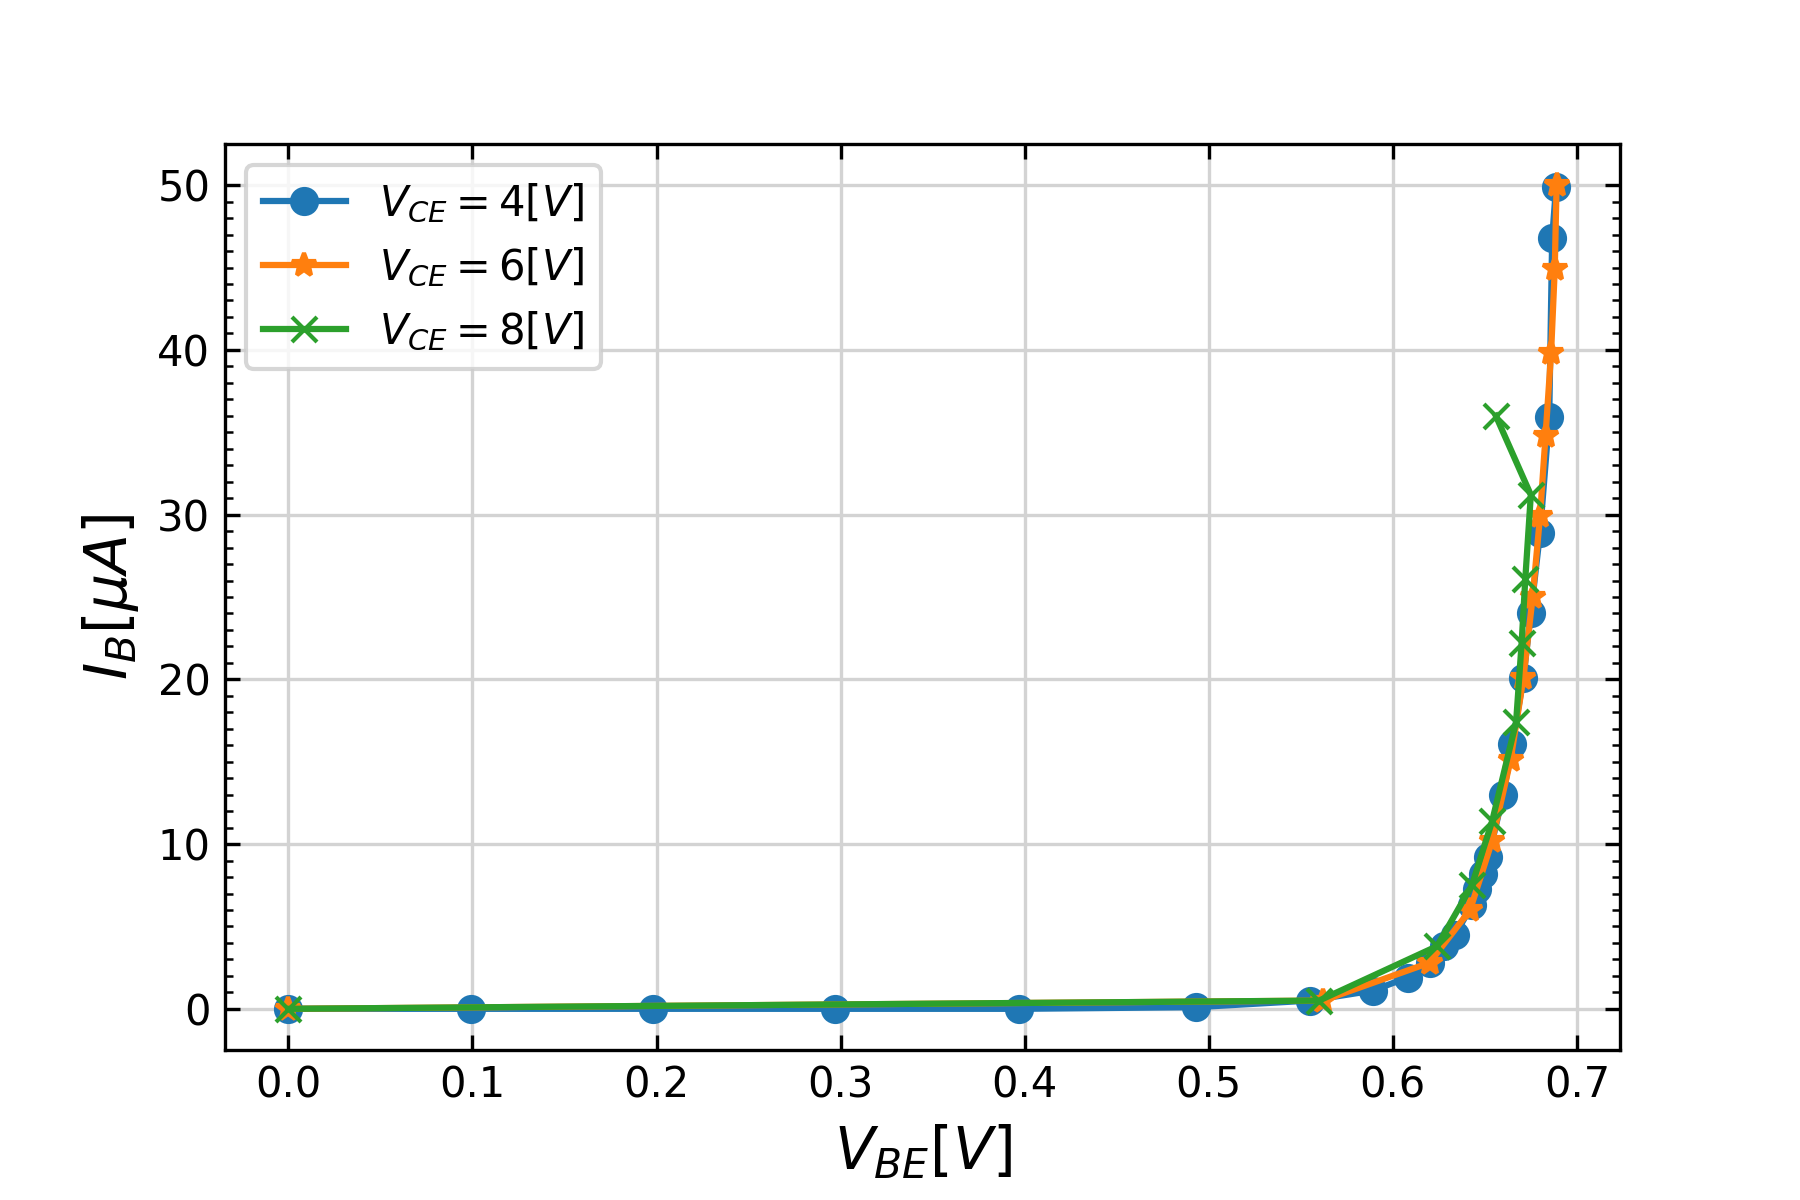
\includegraphics[height=55mm]{ex-1.png}
        \caption{$Tr_1$の入力特性}
        \label{ex:1}    
    \end{figure}
    
    \newpage
    以下表\ref{tbl:2}に$Tr_2$の測定結果の表を,図\ref{ex:2}に$Tr_2$の測定結果のグラフを示す.
    \begin{table}[H]
        \centering
        \caption{$Tr_2$の入力特性の測定値}
        \label{tbl:2}
        \small
        \begin{tabular}{|l|l|l|l|l|l|}
        \hline
        \multirow{2}{*}{$V_{BE}[V]$} & $V_{CE}=4[V]$ & \multirow{2}{*}{$V_{BE}[V]$} & $V_{CE}=6[V]$ & \multirow{2}{*}{$V_{BE}[V]$} & $V_{CE}=8[V]$ \\ \cline{2-2} \cline{4-4} \cline{6-6} 
                                & $I_B[\mu A]$   &                         & $I_B[\mu A]$   &                         & $I_B[\mu A]$   \\ \hline
        0                       & 0        & 0                       & 0        & 0                       & 0        \\ \hline
        0.099                   & 0        & 0.562                   & 0.5      & 0.56                    & 0.5      \\ \hline
        0.198                   & 0        & 0.62                    & 2.8      & 0.624                   & 3.8      \\ \hline
        0.297                   & 0        & 0.642                   & 6        & 0.643                   & 7.5      \\ \hline
        0.397                   & 0        & 0.654                   & 10.2     & 0.654                   & 11.4     \\ \hline
        0.493                   & 0.1      & 0.664                   & 15.1     & 0.667                   & 17.4     \\ \hline
        0.555                   & 0.5      & 0.671                   & 20.1     & 0.67                    & 22.2     \\ \hline
        0.589                   & 1.1      & 0.676                   & 25       & 0.672                   & 26.1     \\ \hline
        0.608                   & 1.9      & 0.68                    & 29.9     & 0.675                   & 31.2     \\ \hline
        0.62                    & 2.8      & 0.683                   & 34.8     & 0.656                   & 36       \\ \hline
        0.628                   & 3.8      & 0.686                   & 39.8     & -                       & -        \\ \hline
        0.634                   & 4.5      & 0.688                   & 44.9     & -                       & -        \\ \hline
        0.643                   & 6.3      & 0.689                   & 50       & -                       & -        \\ \hline
        0.646                   & 7.3      & -                       & -        & -                       & -        \\ \hline
        0.649                   & 8.2      & -                       & -        & -                       & -        \\ \hline
        0.652                   & 9.2      & -                       & -        & -                       & -        \\ \hline
        0.66                    & 13       & -                       & -        & -                       & -        \\ \hline
        0.665                   & 16.1     & -                       & -        & -                       & -        \\ \hline
        0.671                   & 20.1     & -                       & -        & -                       & -        \\ \hline
        0.675                   & 24       & -                       & -        & -                       & -        \\ \hline
        0.68                    & 28.9     & -                       & -        & -                       & -        \\ \hline
        0.685                   & 35.9     & -                       & -        & -                       & -        \\ \hline
        0.6866                  & 46.8     & -                       & -        & -                       & -        \\ \hline
        0.6887                  & 49.9     & -                       & -        & -                       & -        \\ \hline
        \end{tabular}
        \normalsize
    \end{table}
    \begin{figure}[H]
        \centering
        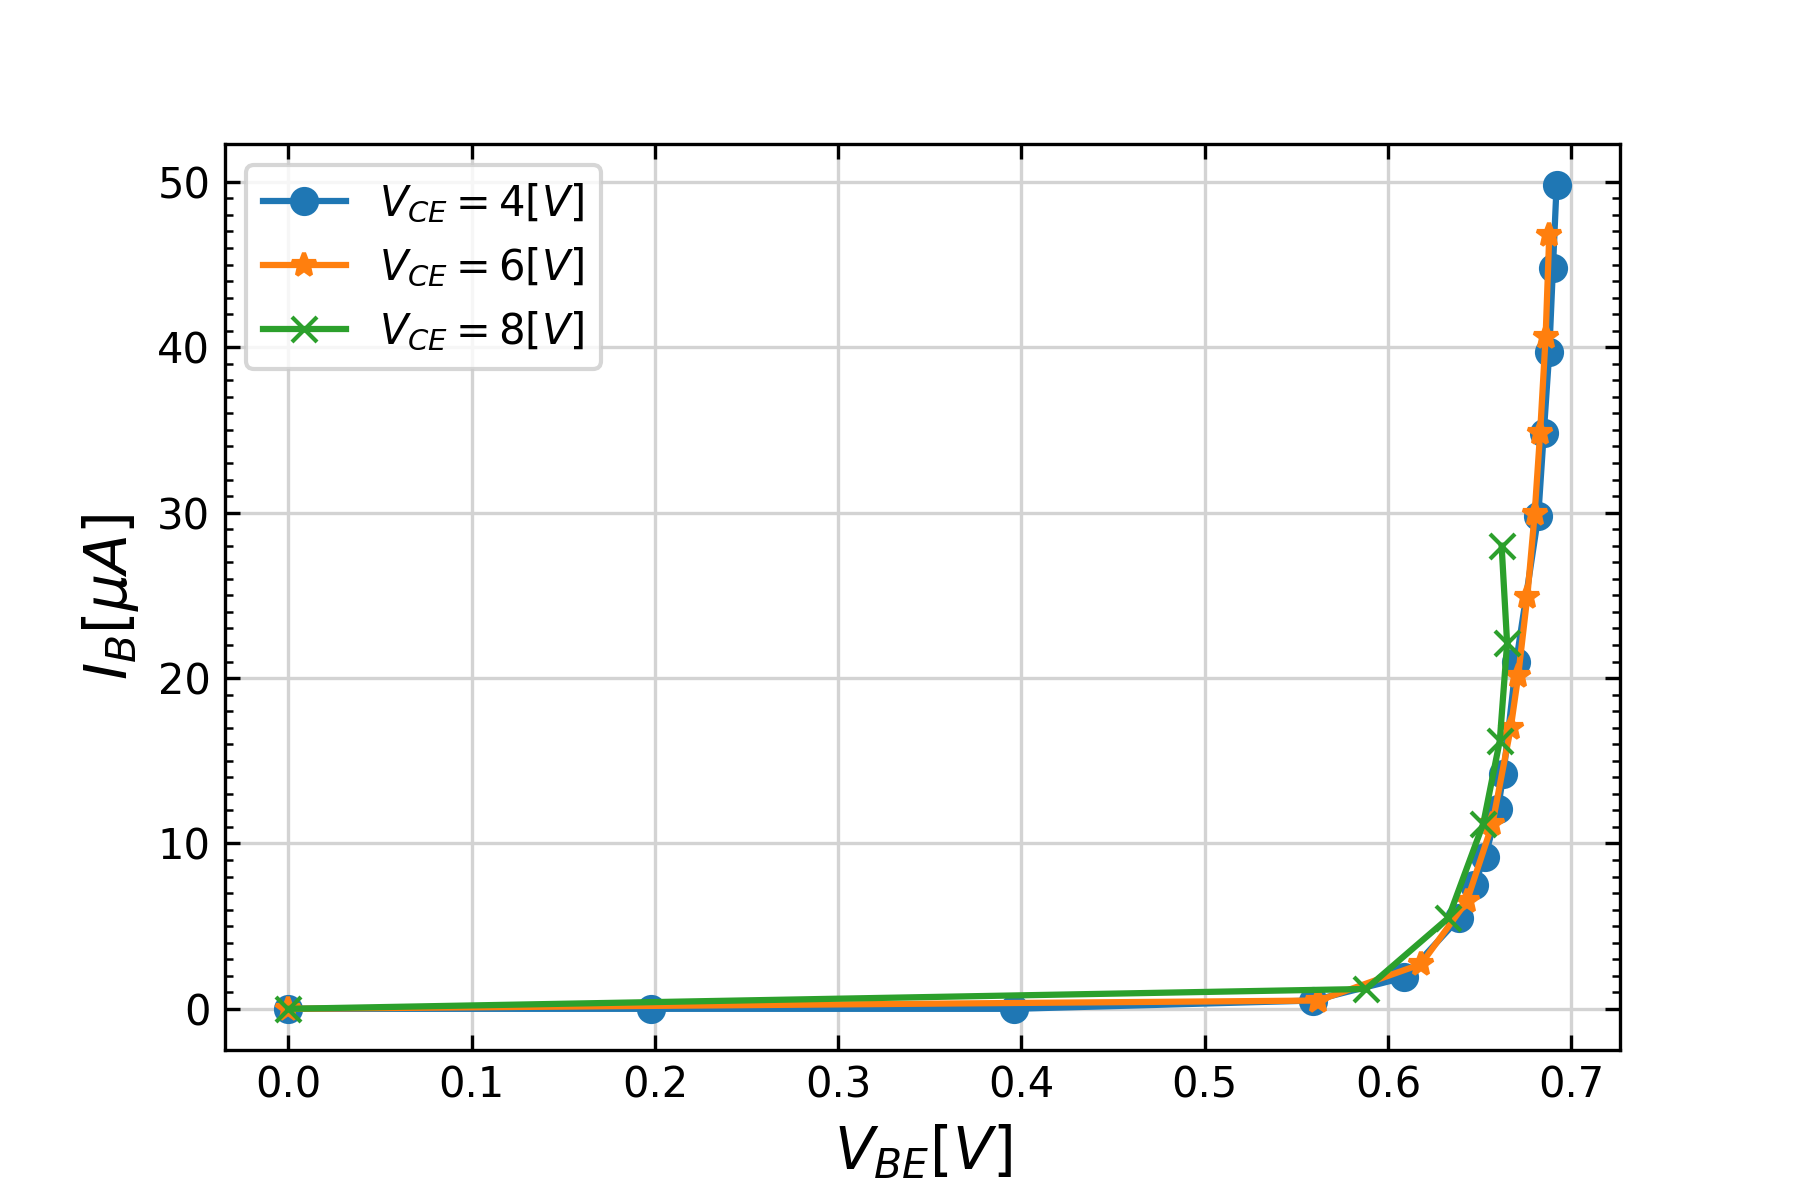
\includegraphics[height=50mm]{ex-2.png}
        \caption{$Tr_2$の入力特性}
        \label{ex:2}    
    \end{figure}

    \newpage
    以下表\ref{tbl:3}に$Tr_3$の測定結果の表を,図\ref{ex:3}に$Tr_3$の測定結果のグラフを示す.
    \begin{table}[H]
        \centering
        \caption{$Tr_3$の入力特性の測定値}
        \label{tbl:3}
        \small
        \begin{tabular}{|l|l|l|l|l|l|}
        \hline
        \multirow{2}{*}{$V_{BE}[V]$} & $V_{CE}=4[V]$ & \multirow{2}{*}{$V_{BE}[V]$} & $V_{CE}=6[V]$ & \multirow{2}{*}{$V_{BE}[V]$} & $V_{CE}=8[V]$ \\ \cline{2-2} \cline{4-4} \cline{6-6} 
        & $I_B[\mu A]$   &                         & $I_B[\mu A]$   &                         & $I_B[\mu A]$   \\ \hline
        0                       & 0        & 0                       & 0        & 0                       & 0        \\ \hline
        0.099                   & 0        & 0.562                   & 0.5      & 0.56                    & 0.5      \\ \hline
        0.198                   & 0        & 0.62                    & 2.8      & 0.624                   & 3.8      \\ \hline
        0.297                   & 0        & 0.642                   & 6        & 0.643                   & 7.5      \\ \hline
        0.397                   & 0        & 0.654                   & 10.2     & 0.654                   & 11.4     \\ \hline
        0.493                   & 0.1      & 0.664                   & 15.1     & 0.667                   & 17.4     \\ \hline
        0.555                   & 0.5      & 0.671                   & 20.1     & 0.67                    & 22.2     \\ \hline
        0.589                   & 1.1      & 0.676                   & 25       & 0.672                   & 26.1     \\ \hline
        0.608                   & 1.9      & 0.68                    & 29.9     & 0.675                   & 31.2     \\ \hline
        0.62                    & 2.8      & 0.683                   & 34.8     & 0.656                   & 36       \\ \hline
        0.628                   & 3.8      & 0.686                   & 39.8     & -                       & -        \\ \hline
        0.634                   & 4.5      & 0.688                   & 44.9     & -                       & -        \\ \hline
        0.643                   & 6.3      & 0.689                   & 50       & -                       & -        \\ \hline
        0.646                   & 7.3      & -                       & -        & -                       & -        \\ \hline
        0.649                   & 8.2      & -                       & -        & -                       & -        \\ \hline
        0.652                   & 9.2      & -                       & -        & -                       & -        \\ \hline
        0.66                    & 13       & -                       & -        & -                       & -        \\ \hline
        0.665                   & 16.1     & -                       & -        & -                       & -        \\ \hline
        0.671                   & 20.1     & -                       & -        & -                       & -        \\ \hline
        0.675                   & 24       & -                       & -        & -                       & -        \\ \hline
        0.68                    & 28.9     & -                       & -        & -                       & -        \\ \hline
        0.685                   & 35.9     & -                       & -        & -                       & -        \\ \hline
        0.6866                  & 46.8     & -                       & -        & -                       & -        \\ \hline
        0.6887                  & 49.9     & -                       & -        & -                       & -        \\ \hline
        \end{tabular}
        \normalsize
    \end{table}
    \begin{figure}[H]
        \centering
        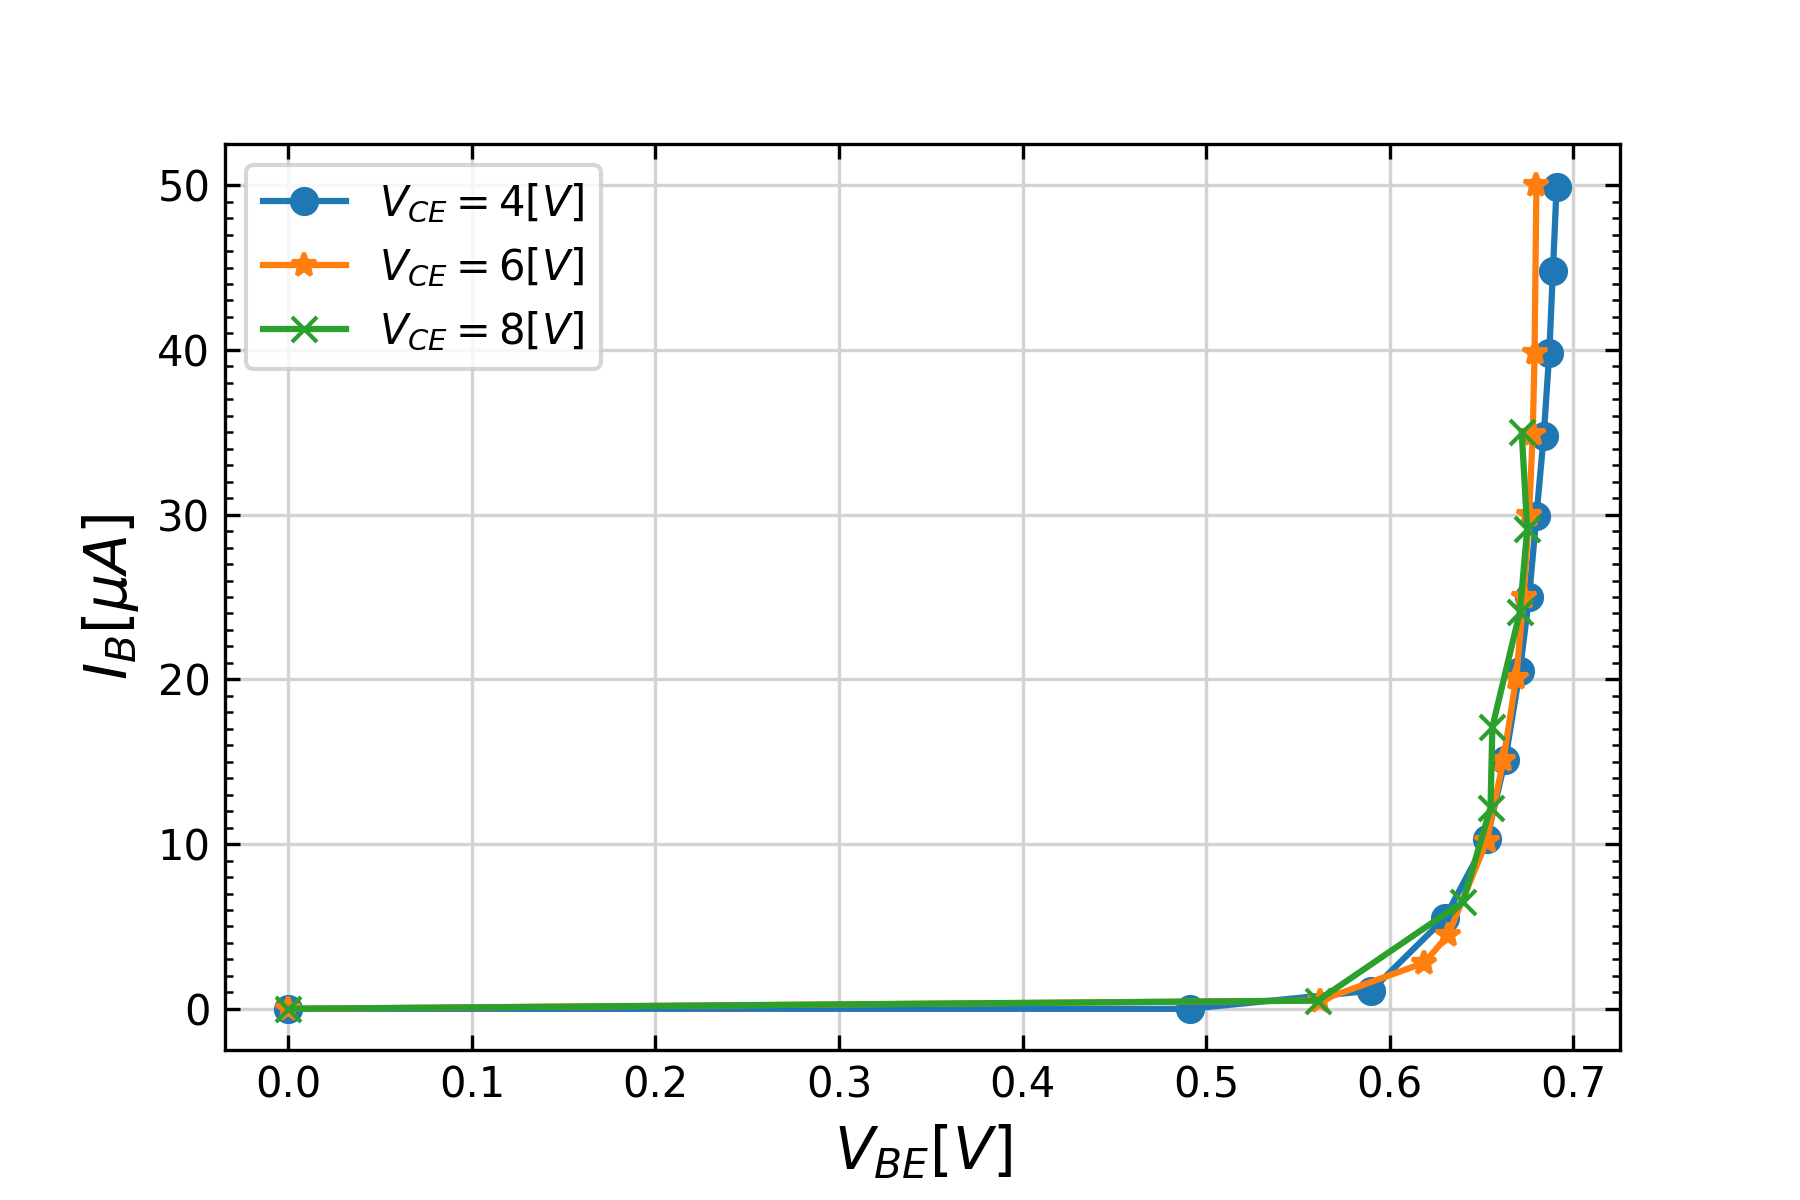
\includegraphics[height=50mm]{ex-3.png}
        \caption{$Tr_3$の入力特性}
        \label{ex:3}    
    \end{figure}

\end{document}